% begin module limit-at-infinity-ex4
\begin{frame}
\begin{example}[Example 4, p. 234]
Find the horizontal and vertical asymptotes of $f(x) = \frac{\sqrt{2x^2+1}}{3x-5}$.
\begin{columns}[c]
\column{.35\textwidth}
\ \only<handout:0| -17>{%
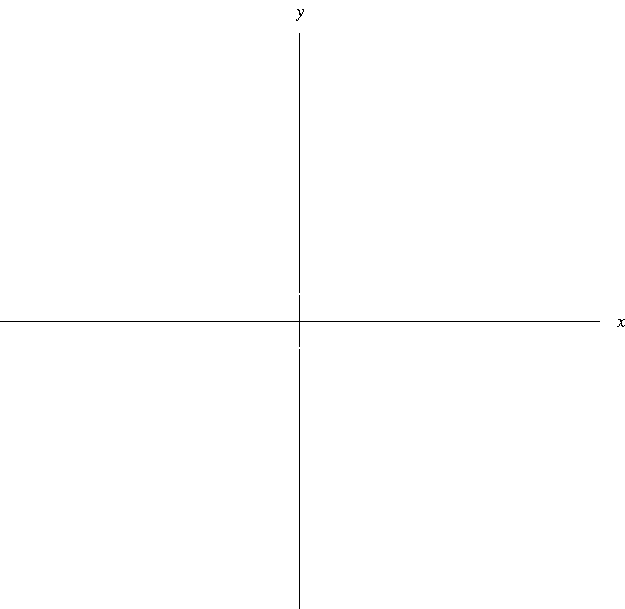
\includegraphics[width=4.5cm]{curve-sketching/pictures/04-04-ex4a.pdf}%
}%
\only<handout:0| 18-21>{%
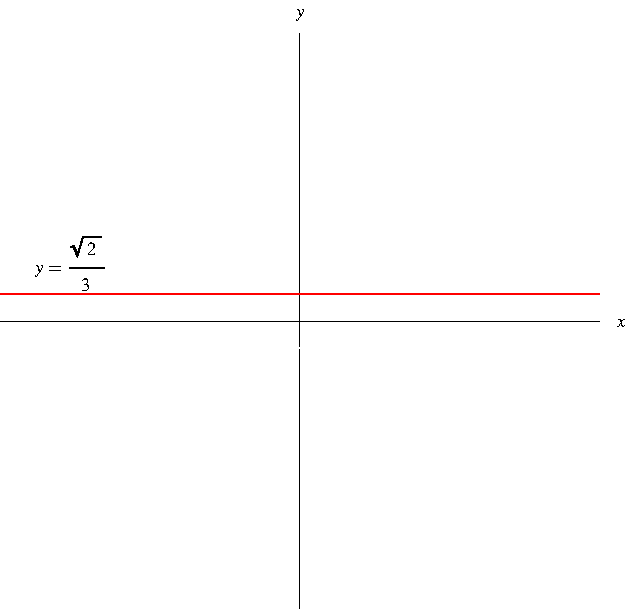
\includegraphics[width=4.5cm]{curve-sketching/pictures/04-04-ex4b.pdf}%
}%
\only<handout:0| 22-23>{%
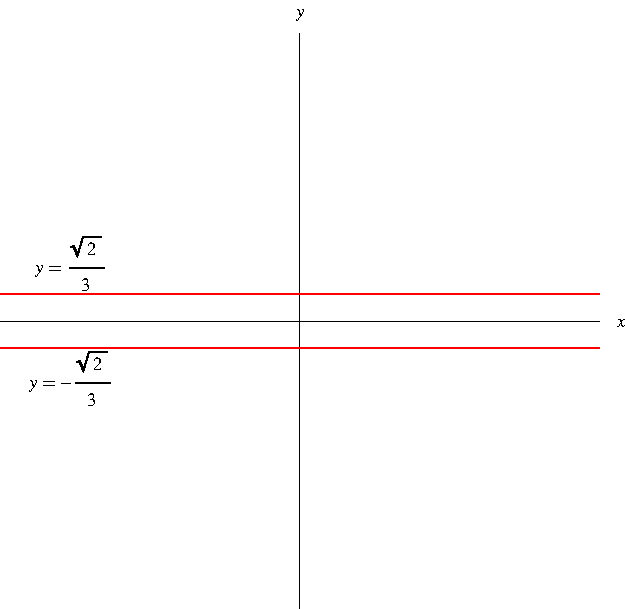
\includegraphics[width=4.5cm]{curve-sketching/pictures/04-04-ex4c.pdf}%
}%
\only<handout:0| 24>{%
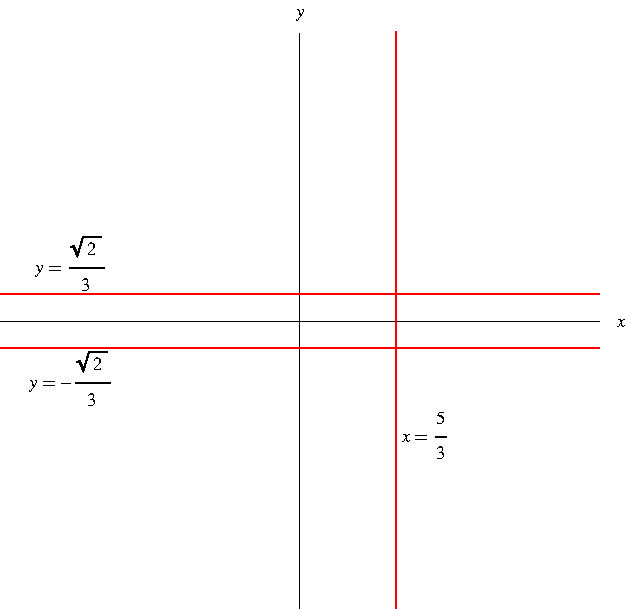
\includegraphics[width=4.5cm]{curve-sketching/pictures/04-04-ex4d.pdf}%
}%
\only<25->{%
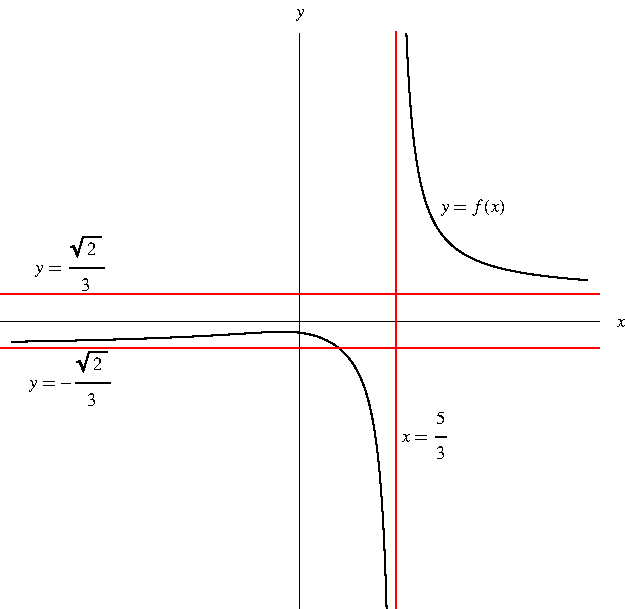
\includegraphics[width=4.5cm]{curve-sketching/pictures/04-04-ex4e.pdf}%
}%
%\begin{itemize}

\uncover<4->{\alertNoH{ 4}{If $x > 0$ then $x = \sqrt{x^2}$.}}

\uncover<20->{\alertNoH{ 20}{If $x < 0$ then $x = -\sqrt{x^2}$.}}

\uncover<23->{\alertNoH{ 23-24}{Vertical Asymptote: \uncover<24->{$x = \frac{5}{3}$.}}}
%\end{itemize}
\column{.65\textwidth}

\abovedisplayskip=0pt
\belowdisplayskip=0pt
\[
\begin{array}{l}
\uncover<2->{%
\displaystyle \lim_{x\to \infty} \frac{\sqrt{2x^2+1}}{3\alertNoH{ 3}{x}-5}\uncover<3->{\alertNoH{ 3}{\cdot \frac{\alertNoH{ 4}{\frac{1}{x}}}{\frac{1}{x}}}}%
}%
%\\%
%& \uncover<4->{ = } &%
\uncover<4->{%
\displaystyle = \lim_{x\to \infty} \frac{\sqrt{\alertNoH{ 5-6}{2x^2+1}}}{\alertNoH{ 7-8}{3x-5}}\cdot \frac{\alertNoH{ 4-6}{\frac{1}{\sqrt{x^2}}}}{\alertNoH{ 7-8}{\frac{1}{x}}}%
}%
\\%
%& \uncover<8->{ = } &%
\uncover<5->{%
\displaystyle = \lim_{x\to \infty} \frac{\sqrt{\alertNoH{ 5-6}{\uncover<6->{2+\frac{1}{x^2}}}}}{\alertNoH{ 7-8}{\uncover<8->{3-\frac{5}{x}}}}%
}%
\uncover<9->{%
\displaystyle = \frac{\sqrt{\displaystyle \alertNoH{ 10-11}{\lim_{x\to\infty}2} + \alertNoH{ 12-13}{\lim_{x\to\infty}\frac{1}{x^2}}}}{\displaystyle \alertNoH{ 14-15}{\lim_{x\to\infty}3} - \alertNoH{ 16-17}{5\lim_{x\to\infty}\frac{1}{x}}}%
}%
\\%
%& \uncover<9->{ = } &%
\uncover<10->{%
\displaystyle = \frac{\sqrt{\uncover<11->{\alertNoH{ 11}{2}} + \uncover<13->{\alertNoH{ 13}{0}}}}{\uncover<15->{\alertNoH{ 15}{3}} - \uncover<17->{\alertNoH{ 17}{0}}}%
}%
\uncover<18->{%
 = \frac{\sqrt{2}}{3}%
}%
\end{array}
\]

\abovedisplayskip=0pt
\belowdisplayskip=0pt
\[
\begin{array}{l}
\uncover<2->{%
\displaystyle \lim_{x\to -\infty} \frac{\sqrt{2x^2+1}}{3\alertNoH{ 19}{x}-5}\uncover<19->{\alertNoH{ 19}{\cdot \frac{\alertNoH{ 20}{\frac{1}{x}}}{\frac{1}{x}}}}%
}%
\uncover<20->{%
\displaystyle = \lim_{x\to -\infty} \frac{\sqrt{2x^2+1}}{3x-5}\cdot \frac{\alertNoH{ 20}{\frac{-1}{\sqrt{x^2}}}}{\frac{1}{x}}%
}%
\\%
\uncover<21->{%
\displaystyle = \lim_{x\to -\infty} -\frac{\sqrt{2+\frac{1}{x^2}}}{3-\frac{5}{x}}%
}%
\uncover<22->{%
\displaystyle = -\frac{\sqrt{2}}{3}
}%
\end{array}
\]

\end{columns}
\end{example}
\end{frame}
% end module limit-at-infinity-ex4
